\section{Related Work}

Given the limited amount of related work in the Linux arena, it is well worth it to look at work that has been done for other operating systems as it may influence our final design. The related work will also act as case studies of current techniques used for detouring.

\subsection{Microsoft Detours}

\textbf{Detours} is a mature proprietary Microsoft library for the Windows operating system which provides functionality for the interception of arbitrary Win32 functions\cite{detours_microsoft_research}. The library only allows detours to be inserted at execution time by modifying memory as with the dynamic approach described earlier. The rationale given for this is that it facilitates interception at a very fine granularity allowing detouring of one running instance of an application whilst another instance of the original application runs alongside. However, this is not an exclusive feature of dynamic detouring since executable editing tools often allow the creation of a new executable.

When Detours was initially released, it introduced trampolining, a feature not seen with other detouring packages released at the time. Other features supplied by Detours are Windows-specific such as the ability to edit import tables of binaries. Detours instruments code extremely efficiently with benchmarks placing interception overheads at less than 400ns on the 200MHz processors the library was initially tested on. Another advantage over binary rewriters is size, with Detours adding less than 18KB to an instrumentation package. However, this comes at the cost of an inability to insert code between instructions or basic blocks. Binary rewriters can typically insert instrumentation arbitrarily by performing sophisticated code analysis with techniques such as register scavenging. On the other hand, Detours relies on matching calling conventions to properly preserve register values at the function level. For example, \textbf{stdcall} designates \textbf{eax}, \textbf{ecx} and \textbf{edx} for use within a function and hence these registers are trashable by instrumentation code. This method would not be appropriate for our case since we require modification at the basic block level where looking solely at the call convention would not help determine free registers.

\subsubsection{Advantages and Disadvantages}

Detours is a lightweight library with a distinctly clean API which has no doubt contributed to its success on the Windows platform. The library is written such that a user can make good use of it with only a superficial understanding of Windows internals. Even though Detours is only available for Windows, we can likely borrow from or at least be influenced by its API if we implement dynamic detouring. From a technical level, Detours works in a similar way to the \emph{LD\_PRELOAD} method we described previously. It performs a very limited amount of static manipulation on the target binary's import section to have it load the DLL (Windows' equivalent of a shared library). Since the details of editing the import section are Windows-specific, we shall not go into it further. However, later we will see the same technique employed on the Linux platform by LEEL.

\subsection{EEL}

\textbf{EEL} (Executable Editing Library) is a library for building tools to analyze and modify compiled executable programs on SPARC systems\cite{eel}. EEL works by removing existing instructions and adding foreign code that observes or modifies the original program's execution. Binary rewriting is non-trivial so it is worth it for us to discuss in more detail the intricacies of this technique. The tool provides five major conceptual abstractions in the form of C++ class hierarchies:

\begin{enumerate}
 \item \textbf{Executable} - This is the top-level abstraction which represents any container of executable code, regardless of the specific format.
 \item \textbf{Routine} - Executables contain many routines, which are discovered by the library through static code analysis.
 \item \textbf{CFG (Control-Flow Graphs)} - A CFG is a directed graph with nodes as basic blocks and edges representing control flow between these blocks. The CFG is also generated through static control-flow and data-flow analysis.
 \item \textbf{Instruction} - Basic blocks are composed of these machine-independent descriptions of opcodes. Each instruction object holds intimate information about what registers is reads/writes, which aids data-flow analysis.
 \item \textbf{Snippet} - Snippets encapsulate the machine-specific foreign code that is to be added (instrumentation code). Snippets also take responsibility for register allocation through the use of register scavenging. Snippets often need to be written in assembly language although the authors argue this is not a drawback because the code is usually short and carefully written for efficiency. Useful work is done by separately inserting user defined routines which the snippets call out to.
\end{enumerate}

The abstractions EEL provide are not merely there to hide the complex and low-level implementation details but more so to provide machine-independence. All static analysis performed by the library is completely machine-independent and is supported by requiring every implementation of the EEL library to contain a separate backend-frontend mapping of architecture-specific instructions to EEL's own representation. Theoretically, the library could be ported to any architecture if the appropriate translations were made from EEL instructions to the machine-specific instructions. However, EEL was originally written for RISC instruction sets such as SPARC and MIPS. For this reason, CISC instructions are difficult to synthesize effectively in terms of EEL instructions. For example, string-manipulation instructions such as \textbf{movs}, \textbf{scas}, etc. do not interact with registers in a trivial way. It is not ideal to model the dynamic behaviour and internal control flow of x86 CISC instructions such as these against classic RISC instructions. One approach is to model a CISC instruction as multiple RISC instructions\cite{intermodule_code_optimization}, but this is inconvenient, complex and exposes underlying implementation details thereby breaking abstractions.

Despite the focus on portability, EEL still has architecture-specific details even within its instruction class due to the non-generic nature of some of its target instruction sets. An example of this is representation for delayed branching which is inherent to SPARC but completely absent in the x86 instruction sets. Details such as these unnecessarily add extra complexity to the final library if we were to port it to x86-32 and x86-64.

The portability in itself is a double-edged sword since EEL has catered for it to such an extent that the library and API has become clunky and complicated in comparison to libraries such as Detours. The last update to the source of EEL was well over a decade ago and it is likely the code is now too outdated to be of feasible use to us. Furthermore, the library is already far too bulky to consider extending and this is driven home by the unacceptable size markup when adding even basic instrumentation code. A simple program written in C with a size of 8KB is bloated to 350KB after insertion of a minimal amount of instrumentation code which simply instruments all routines to print their names\cite{leel}. The reason for this is that EEL inserts code from an object file containing the new routines. Since it is unknown whether these routines call sub-routines, the whole object file is inserted. One of the requirements for our tool is that it must be lightweight and have minimal impact to performance so we must avoid this problem in our final solution.

\subsubsection{Advantages and Disadvantages}

EEL presents a complete system for executable editing even though it is too vast to be of direct use to us. Despite this, it is interesting to consider the concept of the machine-independent representation which adds a layer of abstraction above machine-specific opcodes and allows the library to be ported to multiple architectures (previous versions also ran on MIPS, but the most recent version works only for SPARC). Some of the more novel design decisions such as the use of CFGs and the use of an abstraction layer are certainly tempting features to include in our implementation if we opt for executable editing. However, we are only considering Linux x86-32 and x86-64, so adding an extra layer of abstraction may not be necessary since the two instruction sets do not differ greatly. Instead, a more appropriate option as an abstraction layer might be to build on top of the BFD library.

\subsection{LEEL}

\textbf{LEEL} (Linux Executable Editing Library) is an executable editing library for Linux systems running on Intel x86-32 processors\cite{leel}. The project was motivated by EEL and the workflow of tools using both libraries are similar. LEEL identifies shortcomings of the original EEL library and addresses them by adapting a new design. The final product closely resembles EEL from a functional aspect so we will discuss mainly the additional features offered by LEEL\footnote{It should be noted that the similarities and differences discussed are concerning LEEL acting upon executables. It is outside the scope of this project to consider editing relocatable object files and shared libraries.}:

\begin{enumerate}
 \item \textbf{Editing of multiple formats} - LEEL supports editing of executables, relocatable object files and shared libraries.
 \item \textbf{Insertion of user defined routines} - Insertion of user defined routines differs significantly to what we have seen with EEL. It is useful to recall that EEL inserted user defined routines by requiring them to be supplied in an object file which was then inserted into the target. Similarly, LEEL recommends users do most of their processing in an external routine instead of in the snippet itself. However, instead of defining the external routines in an object file, LEEL requires the routines to be contained in a shared library. As we will see later, this is a similar approach to that taken by Etch.
 \item \textbf{Insertion of snippets to CFG} - Snippets in EEL need to be written as small chunks of assembly, but LEEL expects most work to be done in external routines. With this expectation, it simply exposes an API which allow users to generate the assembly code for common tasks such as calling an external routine.
 \item \textbf{Lightweight} - One of the problems with EEL was the huge file bloat after the injection of user-defined routines. Files generated by LEEL have a small overhead in comparison (a sample program with an original size of 11KB is increased to less than 17KB). The problem was solved by having users compile their routines into a shared library and calling out to these routines from instrumented code. A side effect of this is that the development of this shared library and the creation of the snippets can be performed independently as long as function names and signatures are agreed upon. Furthermore, after the new executable is generated, the shared library can be continually updated without requiring further executable editing as long as it continues to adhere to the mutually accepted function names and signatures.
\end{enumerate}

\begin{figure}[H]
 \centering
 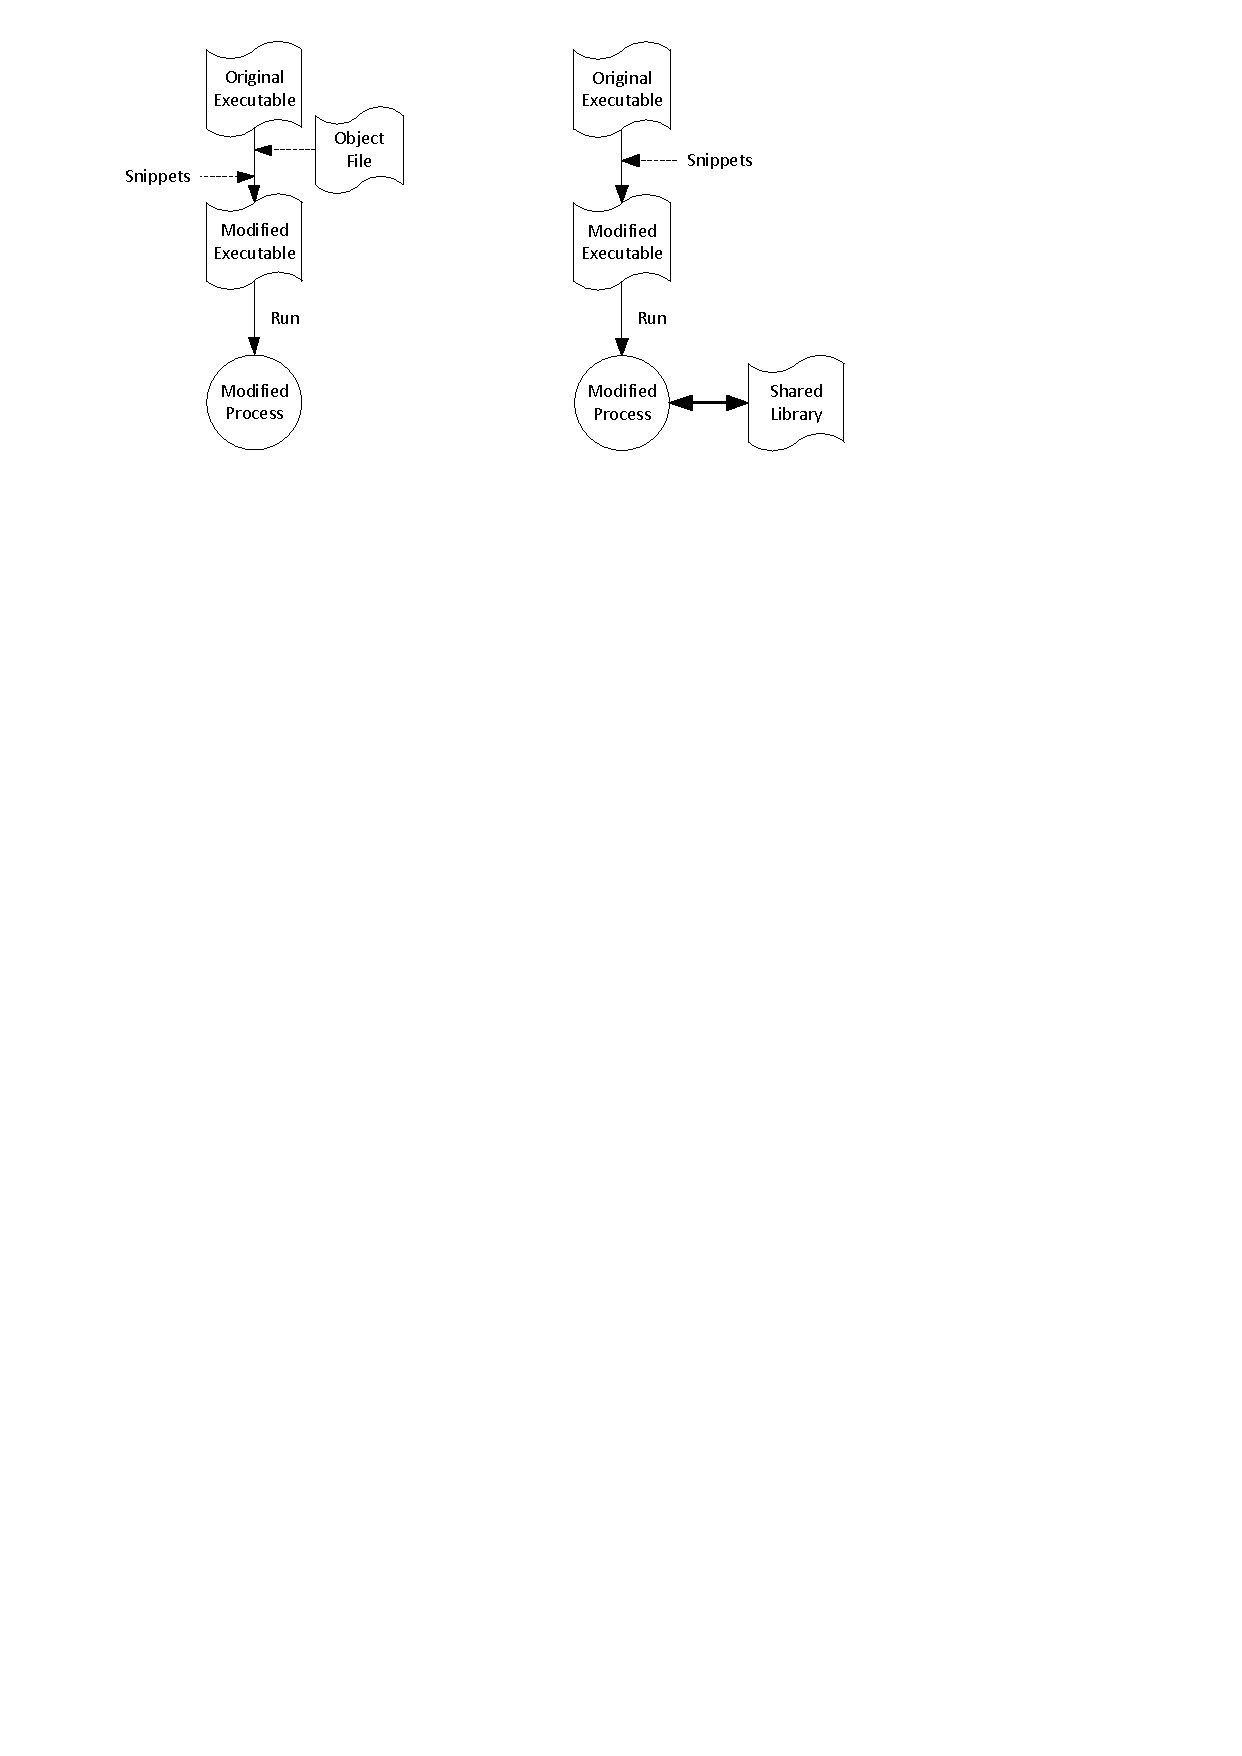
\includegraphics[viewport=60 624 406 825]{LEEL_vs_EEL.pdf}
 \caption[LEEL vs EEL]{The left-hand side shows an executable being modified by EEL. An object file is inserted containing user-defined routines. Snippets allow the original code to be modified to make use of the new routines. The right-hand side shows the same process via LEEL. Snippets are inserted to make use of external routines in a shared library. The shared library is made available at runtime.}
\end{figure}

The only major stage we did not elaborate on is the static analysis stage of LEEL. As with EEL, the library must perform duties before modification of code occurs. Namely, routines need to be identified and a CFG generated - code flow analysis. However, it is uninteresting to delve deep into this since the process does not differ substantially from EEL. The main difference is in the data flow analysis, which LEEL does not perform at all. The justification for this is that with EEL, snippets are expected to be highly optimized and carefully written and this is why register scavenging is performed (which requires data flow analysis). With LEEL, the focus is less on the snippets and more on the external routines so the code is simply wrapped in \textbf{PUSHAD}/\textbf{POPAD} to automatically save and restore the registers. Register scavenging is also less valuable on the Intel processor because of the relatively few number of registers in comparison to SPARC and is not worth the extra complexity of analysis attributed to a more complex instruction set. One midway alternative that LEEL could have used is matching call conventions as part of the agreed external routine signatures, which would inherently allow the snippet to know which registers were used in the external routine. This is the technique used by Detours.

\subsubsection{Advantages and Disadvantages}

While LEEL offers many desirable features, it has a fundamental abstraction design which is unsuitable for us. The library achieves this by building on top of the ELF library. This was a deliberate design decision and reflects one of the key differences in the aims of the two libraries. Whereas one of EEL's main focuses was portability, LEEL intended only to achieve portability to Win32. Since there exists no backend port of BFD to Win32, this resulted in the decision to work directly with ELF instead. Porting LEEL to use BFD as an abstraction layer is infeasible. It would require almost entirely reprogramming the backend and it would take a lot of effort to avoid breaking the support for the specific cases of relocatable object files and shared libraries. In fact, even porting the library to support x86-64 would be very tough because of the tight coupling against the x86-32 instruction set. As a minor point, LEEL also does not support trampolining although this would not be overly difficult to implement. Despite these drawbacks, LEEL presents good solutions to the same drawbacks we identified with the EEL library.

Executable editing is a complicated process and both EEL and LEEL recognise this by demonstrating huge efforts to minimize the amount of code instrumented directly to the target (snippets) by allowing the compilation of the majority of the code (user defined routines) to be performed separately by the compiler. This code is then integrated at two different stages, either by merging the object file with the executable statically (EEL) or merging the code in the form of a shared library at runtime (LEEL). Overall, LEEL can get away with performing less binary rewriting by shifting the focus to the external routines, but the price for this is that it needs to deal with the additional complexities of:

\begin{enumerate}
 \item \textbf{Modifying the executable to use the shared library} - The target has to be modified to act as if it had originally been dynamically linked to the shared library. This process involves an intimate understanding of the file format.
 \item \textbf{Calling of external routines from snippets} - The snippets must deal with the complexities of interacting with the position independent code of the shared library, where the absolute address of the external routines is not known statically.
\end{enumerate}

\subsection{Etch}

\textbf{Etch} is a general-purpose tool for rewriting arbitrary Win32/x86 binaries without requiring source code\cite{etch}. Binary rewriting under the Win32 environment poses complications which are not present in UNIX-based environments due to system-specific features. It is outside the scope of this project to discuss such challenges, so we shall omit them from this report and focus on the higher level concepts of Etch.

Unlike EEL, Etch weaves the instrumentation phase tightly with the code discovery phase, but uses a separate analysis stage. Etch defines two phases: an instrumentation phase and an analysis phase. The instrumentation phase represents the insertion of instrumentation and modification of the program and the analysis stage represents the program at runtime. A tool created using Etch is similarly split into an instrumentation module and an analysis module with the analysis module being loaded with the executable at runtime. An approximation of the workflow is:

\begin{enumerate}
 \item \textbf{Code Discovery} - Etch performs static code analysis to discover the components of the program. \emph{Figure \ref{fig:EtchHierarchy}} illustrates how Etch views the program hierarchy.
 \item \textbf{Callback} - The instrumentation module supplies a callback which Etch calls upon discovery of each component. Each invocation of the callback provides an opportunity to insert instrumentation or modify the executable. This modification can happen at the instruction, basic block or procedural level. Inserted instructions may include calls to procedures in the analysis module.
 \item \textbf{Executable Generation} - The complete traversal of the executable concludes the instrumentation stage and a new executable is generated.
 \item \textbf{Running the Executable} - The executable is run alongside the analysis module. Etch provides a hook providing notification to the analysis module of program completion. The module can then optionally run some analysis routines based on data collected during execution.
\end{enumerate}

\begin{figure}[H]
\Tree[.Program [.Module [.Procedure [.{Basic Block} Instruction {\ldots} ] {\ldots} ].{Procedure}
      {\ldots} ].Module {\ldots} ]
\caption{Etch views a program as a collection of modules. Each module contains procedures, which are composed of basic blocks which in turn are composed of instructions.}
\label{fig:EtchHierarchy}
\end{figure}

Etch provides additional features which are less related to executable editing. For example, it provides facilities to rewrite an executable in order to improve its performance by reordering instructions to optimize code layout to take advantage of spatial and temporal locality. This is a relatively complex example and application of data flow analysis alongside executable editing.

\subsubsection{Advantages and Disadvantages}

Etch presents a vastly different front-end interface compared to EEL, working less directly through the callback system established in the instrumentation module. Since Etch is not an open source project (nor even publicly available), to some extent, we can only speculate about the underlying implementation of the tool. However, it would appear that the separation of `instrumentation' and `analysis' simplifies the task of the editor slightly. By mapping the analysis module in at runtime, calls from the instrumentation can be dynamic which lightens the workload of the executable editing part of the tool by decreasing the amount of code that needs to be injected statically. Essentially, the task of code injection is partially delegated to the OS loader to be performed at runtime, which makes Etch more of a static/dynamic hybrid rather than a strict static binary rewriter.

Aside from the technical ramifications, the separation of the two duties reflects a different approach to the creation of a tool through Etch. It allows a user to treat the analysis module as a library and also decouples the instrumentation from the logic of analysing the data gleaned at runtime. In a way, this is more natural than the approach taken with EEL which tends to focus on the injection of small and optimized snippets of code.

\subsection{ELFsh}

\textbf{ELFsh} is an interactive, modular, and scriptable ELF machine for static binary instrumentation of executable files, shared libraries and relocatable ELF objects\cite{elfsh}. ELFsh differs from most other implementations in that it does not come in the form of a library nor does it provide a programmatic interface other than in the form of a scriptable command-line. The main way to use ELFsh is interactively through the command prompt. The tool provides access to many low-level features such as reading and writing of ELF sections and symbol tables. However these features are not only file-format specific, but also do not directly provide useful functions to an end-user and should be abstracted in our tool. The reason these features are available in ELFsh from the user-level is mainly because of the implementation approach taken. From a high-level, ELFsh provides the following features:

\begin{enumerate}
 \item \textbf{Injection of instrumentation} - The instrumentation must be in the form of an object file and is added into the target as if the binary has not been linked yet. Internally, this works by adding a library dependence to the main object\cite{cerberus_elf}.
 \item \textbf{Function redirection} - By exploiting the way that dynamically linked function calls are resolved, existing procedures can be hijacked. When resolving symbols, the runtime linker iterates over a \emph{link\_map} list and resolves each symbol to an absolute runtime address where the function is mapped. By forcing some symbols to be resolved in priority, ELFsh is able to control the procedures to which symbols resolve to. ELFsh does not provide convenient access to the original function. Instead, the common practice to access it is to call \texttt{dlopen} and \texttt{dlsym} in the hook function. This allows a function address to be resolved at runtime based off a module and function name.

\end{enumerate}

\subsubsection{Advantages and Disadvantages}

ELFsh demonstrates less conventional techniques for the binary rewriting process, which is due to its birth in the reverse engineering scene. For the most part, the tool is able to avoid dealing with concepts such as static code analysis by relying on pre-existing analysis from the user. For example, it provides no function to enumerate procedures so the parameters to \texttt{dlopen} and \texttt{dlsym} would have to be determined beforehand at the compile-time of the instrumentation object file. The tool is able to discover such information interactively but the lack of a proper programmatic interface makes the process much more manual. The tool is unsuitable for us for various other reasons:

\begin{enumerate}
 \item \textbf{Lack of abstraction layer} - As discussed earlier, one of our primary irks with ELFsh is the fact that it is built on top of libelf. This is exploited by using file-specific tricks to implement the features provided by the tool. The tool pays the price for this in portability, with ports requiring manual porting of the backend. The difficulty of this is evidenced in the fact that despite ports existing to other architectures, only the Intel version is fully featured.
 \item \textbf{Lack of granularity} - ELFsh lacks the granularity and control given with other binary editing tools. It does not allow the insertion of instrumentation at the instruction level, nor even at the basic block level. Another granularity related problem is that due to the nature of the injection (entire object file injected), the tool faces similar size markup issues as seen with EEL.
 \item \textbf{Development state} - ELFsh is an old project that is no longer maintained or developed.
\end{enumerate}

One concept we can take away from ELFsh is the scriptable command-line. Even though we want to create a library, it would be nice to be able to operate our tool through a command-line also.

\subsection{Pin/DynamoRIO}

\emph{Pin} and \emph{DynamoRIO} are two tools which perform run-time binary instrumentation of Linux and Windows applications\cite{pin,pin_windows,dynamorio}. The two tools are completely separate but due to the similarities of their implementation they have been grouped together here. We will talk about Pin, but the concepts are applicable to both tools unless explicitly stated.

Pin does not make any static modifications to the executable. Instead, it uses \emph{dynamic recompilation} to run the target in a process-level virtual machine which intercepts execution at the entry point and injects a runtime agent which performs the insertion of the instrumentation. 

Pin is used to create an architecture independent Pintool which can access architecture-specific details when necessary. The Pintools are written in C/C++ making them theoretically source compatible across different architectures. Pin is viewed as an efficient solution compared to other runtime detouring implementations because of its use of just-in-time (JIT) compiling to insert and optimize code.

\subsubsection{Advantages and Disadvantages}

The advanced process-level virtual machine Pin utilizes requires the distribution of a substantial environment so is not quite suitable for us. However, interception from this level allows for a high level of observability which is usually difficult to obtain. Whereas the tools we have looked at so far operate mostly at the instruction, basic block and procedural level, Pin allows higher level abstractions to be observed. For example, instrumentation can be notified upon events such as loading/unloading of shared libraries and creation/end of threads. It is possible to reproduce these effects with regular tools by detouring system library functions but this convenience and ease of use is one of Pin's selling points. If we have time, it would be good to mimic this concept of moving more responsibility from the user to the library.

Pin takes full advantage of the flexibility offered by dynamic detouring presenting features such as process attaching and detaching. Pin suffers from the overhead inferred from runtime attachment, but makes up for it with its powerful JIT compiler. Firstly, by performing code discovery at runtime, Pin is able to gather more comprehensive information about the program compared to using static control flow analysis. This extra information allows the tool to perform optimizations on instrumentation which previously had to be done by the user. Secondly, the JIT instruments code on the fly by taking the native executable as input and intercepting its execution, generating new code from it (which is cached) and transferring the target's execution to the generated sequence. Instrumentation can easily be inserted during the translation phase. This process essentially optimizes the code on the fly with the further advantage that the system can reflect the target's runtime environment accurately reducing any effects on the original program's behaviour.

Pin was designed with observation in mind, rather than modification. It can modify the behaviour of the executable by modifying registers and memory but its ability to do so is more limited than some of the other tools we have looked at. In a way, Pin has taken the typical inspections that users might make with regular detouring tools and made these accessible features as part of its API.

\subsection{IDA Pro}

\emph{IDA Pro} is a popular commercial disassembler supporting a large variety of architectures and operating systems\cite{ida,stripped_binary}. The focus with IDA Pro is not on the instrumentation phase, but rather on the automatic code analysis that it performs. The tool is able perform instrumentation, but since it does not present anything substantially different to what we have already seen, we shall draw our comparisons about its ability to perform static analysis.

\subsubsection{Advantages and Disadvantages}

As with all static binary rewriters, IDA Pro faces the problem of discovering functions that are only reachable through indirect control transfer. What is interesting in this case is not what IDA Pro provides, but what it lacks and how it contrasts with solutions provided by other tools.

IDA Pro and EEL both do not provide any support for discovery of functions that are reached via indirect calls. These functions become gaps in the code. LEEL approaches the problem by starting analysis from the program's entry point and recursively building a call graph (same so far). However, it provides two options to deal with the gaps\cite{leel}: either not to analyze them at all or assume that the first byte of a gap is the starting address of a function. It can be argued that this provides two extremes, providing either low code coverage or a high chance of incorrect analysis of non-code blocks as functions. Other tools such as RAD\cite{rad} take the more aggressive approach but use conservative heuristics to prevent false positives such as only analysing blocks if it starts with a known prologue. If we perform static analysis, we will need to take these methods into account and select one appropriately.

\subsection{Others}

There exist various other noteworthy libraries and tools which either perform detouring or make use of it including \emph{Valgrind}, \emph{IDtrace}, \emph{radare2}, \emph{qpt}, \emph{ATOM} and \emph{pixie}\cite{valgrind,IDtrace,radare2,qpt,atom,qpt_pixie}. However these tools do not introduce significant concepts or techniques interesting to us that we have not already seen so we shall not be covering them in further depth.